\documentclass[runningheads,a4paper]{llncs2e/llncs}

\usepackage{amssymb}
\setcounter{tocdepth}{3}
\usepackage{graphicx}
\usepackage{subfigure}
\usepackage{multirow}
\usepackage{amsmath}

\usepackage{algorithm} %for Pseudo code
\usepackage{algorithmic} %for Pseudo code algorithmicx
\renewcommand{\algorithmicrequire}{\textbf{Input:}}  % Use Input in the format of Algorithm
\renewcommand{\algorithmicensure}{\textbf{Output:}} % Use Output in the format of Algorithm
\usepackage{booktabs}
\newcommand{\ra}[1]{\renewcommand{\arraystretch}{#1}}
\newcommand{\tabincell}[2]{\begin{tabular}{@{}#1@{}}#2\end{tabular}}


\begin{document}

\mainmatter  % start of an individual contribution

% first the title is needed
\title{Review Extraction via Mining Microblogs}

% a short form should be given in case it is too long for the running head
\titlerunning{Review Extraction via Mining Microblogs}

% the name(s) of the author(s) follow(s) next
%
% NB: Chinese authors should write their first names(s) in front of
% their surnames. This ensures that the names appear correctly in
% the running heads and the author index.
%
\author{Weiyue Huang
\and Chenhao Zhu
\and Kan Ren}
%
\authorrunning{W. Huang\and C. Zhu and K Ren}
% (feature abused for this document to repeat the title also on left hand pages)

% the affiliations are given next; don't give your e-mail address
% unless you accept that it will be published
\institute{Shanghai Jiao Tong University, Shanghai, China\\
\{hwy, chzhu, kren\}@apex.sjtu.edu.cn \\
}
%
% NB: a more complex sample for affiliations and the mapping to the
% corresponding authors can be found in the file "llncs.dem"
% (search for the string "\mainmatter" where a contribution starts).
% "llncs.dem" accompanies the document class "llncs.cls".
%

\toctitle{Review Extraction via Mining Microblogs}
\tocauthor{W. Huang et al.}
\maketitle


%\begin{abstract}
%
%
%\keywords{}
%\end{abstract}

\section{Introduction}
Recently, social trend becomes more and more obvious in our daily life.
Almost every app or website develops their social module to activate the user community.
Large number of people read articles, communicate, post ideas and find other persons on social media sites.

Social Network (SN) produce great volume of data every day.
In the report\footnote{http://www.theregister.co.uk/2012/11/09/facebook\_open\_sources\_corona/}, some large social media digest petabyte level of information in one day.
Moreover the information produced by SN contains great value.

However, mining social media data requires some professional techniques.
Machine learning algorithms may help to discover latent patterns in social media data.
There are some applications in this field. Pattern mining such as association rules\cite{agrawal1993mining} is used for user browsing behavior mining.
Clustering methods (e.g. K-means) are applied in interest group finding. Recommender systems are built in many e-commerce websites\cite{koenigstein2011yahoo}.
IR techniques are used for product review extraction and clustering\cite{tsaparas2011selecting}.

As is known, there is gigantic volume of valuable information in SN.
Many people may find whatever they want in SN.
However, noise information is filled in data flows of SN.
Algorithms should be well designed to filter out noise while preserving useful information.
Moreover, the information should be cleaned and help to make more value in the future.

Our goal is to find actual review comments about some real things (e.g. restaurants) posted in SN and discard advertisements, meaningless articles or any other noisy information.
We focus on Weibo\footnote{http://www.weibo.com} website which is one of the largest SN in China.
We apply 3 models (SVM, Naive Bayes and Decision Tree) for review classification.
Different features such as mutual information, topic modeling are used to capture the latent information of data.
We also compare the performance of different models with different parameters.
Experiments show comprising results of our system.

\section{Task}
Microblog Review Extraction task is to find real reviews for restaurants in microblog data and filter out noise.
Given a set of microblogs, our system will judge whether each microblog is a real review.

\section{Dataset}
The dataset which we used in this project is collected from Weibo website, one of the largest social network website in Chine.
The dataset contains 123,136 microblogs along the time line with some related information such as id, time, publishing device, number of people who retweet the weibo and POI (��Point of Interest��). And the contents of microblogs are segmented by general segmentation tool.
We also manually labeled 8,498 of them whether a microblog is a review or not.
In this project, a K-fold cross validation method is used to improve our experiment result.

Details of our data set is shown in Table \ref{tab:dataset}.

\begin{table}\centering{
\caption{Data set and examples}
\label{tab:dataset}
\begin{tabular}{ | c | p{7cm} | c | }
\hline
Name & Description & Example \\ \hline
weiboId & the id of the weibo & M\_Blu8QBwGG \\ \hline
like & the number of people who like this weibo & 0 \\ \hline
retweet & the number of people who retweet the weibo & 1 \\ \hline
comment & the number of the comments of the weibo & 0 \\ \hline
pic & pictures in the weibo & 1\\ \hline
POI & Point of Interest & B20\ldots55 (in short) \\ \hline
from & the device from which the weibo is published & iPhone Client \\ \hline
time & the publish time of the weibo & 2014-11-22 08:00:00.0 \\ \hline
content & segmented weibo content & Icecream is so delicious \\ \hline
\end{tabular}
}
\end{table}

\section{Features}
From the dataset, we get several features about a microblog text. To make the most of these features, we pay more attention to the most important one, which is the content of a microblog text.
In our work, we adapt several feature selection methods which are commonly used in text categorization.
\subsection{Mutual Information}
Given a category c and a term t, let A denote the number of times c and t co-occur, B denotes the number of times t occurs without c, C denotes the number of times c occur without t, and N denotes the total number of documents in c. The mutual information criterion between t and c is defined as Equation \ref{equ:1}:

\begin{equation}
\label{equ:1}
  MI(t,c)=\log{\frac{P(t,c)}{P(t)\times P(c)}}
\end{equation}

and is estimated using Equation \ref{equ:2}:

\begin{equation}
\label{equ:2}
  MI(t,c)\approx \log{\frac{A\times N}{(A+C)\times (A+B)}}
\end{equation}

These category-specific scores of a term are then combined to measure the goodness of the term at a global level. Let \{$c_{i}$\}$_{i=1}^{m}$ denote the set of categories in the target space. Typically it can be calculated as Equation \ref{equ:3}.\cite{xu2007study}

According to \cite{church1990word}, the mutual information compares the joint probability of observing t and c together with the probabilities of observing t and c independently. $MI(t,c)$ has a positive value when there is a genuine association between t and c. It has a zero value when there is no significant relationship between t and c and a negative value when t and c are in complementary distribution.

\begin{equation}
\label{equ:3}
  MI_{avg}(t)=\sum_{i=1}^m{P(c_i)MI(t,c_i)}
\end{equation}

In our method, after the computation of these criteria, thresholding is performed to achieve the desired degree of feature elimination from the full vocabulary of a document corpus. Here we use Equation \ref{equ:4} to formulate it.

\begin{equation}
\label{equ:4}
  \bigcup_{i=1}^m \{t|MI(t,C_i)\ is\ the\ top\ K\ largest\ ones\ in\ \{MI(W,c_i)\}\}
\end{equation}

\subsection{Topic Modeling}
In machine learning and natural language processing, the topic model is a type of statistical model for discovering the abstract ``topics'' that occur in a collection of documents\footnote{http://en.wikipedia.org/wiki/Topic\_model} (microblogs).
Intuitively, given that a document is about a particular topic, one would expect particular words to appear in the document more or less frequently.

A document typically concerns multiple topics in different proportions.
In our settings, we use topic modeling method to discover several abstract ``topics" contained inside microblogs.
Then we try to estimate topic probability distributions of given microblogs (i.e. documents).
We could obtain a feature vector after inference topic distribution for each microblog.

We note the feature vector as $\vec{x}_i = (x_1, x_2, \ldots, x_k, \ldots, x_K)^T$ where $K$ is the number of topics and $\vec{x}_i$ is the feature of the $i$th microblog.
Each element in the vector is a probability of a specific topic with regard to the microblog.
Here $x_k = P(t_k|m_i), k=1,2,\ldots,K$.

After generation of feature vectors for the microblogs in the train dataset, we use some classification method to classifiy microblogs (as whether thie microblog is a real revew or not).
In our experiments, we use Support Vector Machine to achieve this goal.

\begin{figure}
\centering
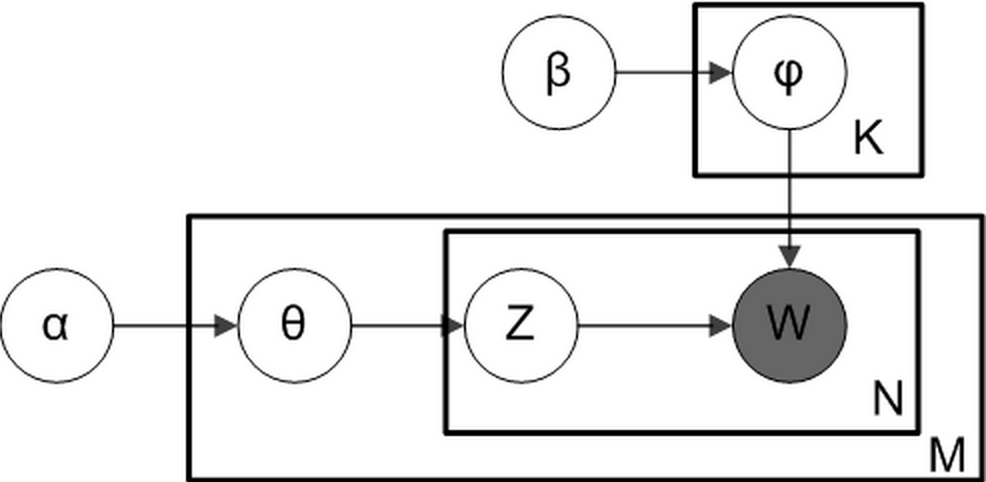
\includegraphics[width=3in]{figures/lda.png}
\caption{Plate Notation of LDA}
\label{fig:lda}
\end{figure}

Figure \ref{fig:lda}\footnote{http://en.wikipedia.org/wiki/Latent\_Dirichlet\_allocation} shows the plate notation of Latent Dirichlet Allocation (LDA)\cite{blei2003latent}.
LDA is a generative model which allows sets of observations to be explained by unobserved groups (latent semantic topics) that explain why some parts of the data are similar.
In our settings,  the observations are words collected in microblogs, it posits that each microblog is a mixture of a small number of topics and that each word's creation is attributable to one of the microblog's topics.

In LDA, the topic distribution is assumed to have a Dirichlet prior.
With plate notation in Figure \ref{fig:lda}, the dependencies among the many variables can be captured concisely.
The boxes are ``plates'' representing replicates.
The outer plate represents microblogs, while the inner plate represents the repeated choice of topics and words within a microblog.

$M$ denotes the number of microblogs, $N$ the number of words in a microblog.
Here $\alpha$ is the parameter of the Dirichlet prior on the per-microblog topic distributions,
$\beta$ is the parameter of the Dirichlet prior on the per-topic word distribution,
$\theta_i$ is the topic distribution for microblog $i$,
$\phi_k$ is the word distribution for topic $k$,
$z_{ij}$ is the topic for the $j$th word in microblog $i$, and
$w_{ij}$ is the specific word.

The $w_{ij}$ are the only observable variables, and the other variables are latent variables.
$\phi$ is a $K\times V$ ($V$ is the dimension of the vocabulary) Markov matrix (transition matrix), and each row of which denotes the word distribution of a topic.

The generative process is as follows. Documents are represented as random mixtures over latent topics, where each topic is characterized by a distribution over words. LDA assumes the following generative process for a corpus $D$ consisting of $M$ microblogs with length $N_i$:
\begin{itemize}
	\item Choose  $\theta_i \,  \sim \, \mathrm{Dir}(\alpha)$ , where  $i \in \{ 1,\dots,M \}$  and  $\mathrm{Dir}(\alpha)$  is the Dirichlet distribution for parameter $\alpha$.
	\item Choose  $\phi_k \, \sim \, \mathrm{Dir}(\beta)$ , where  $k \in \{ 1,\dots,K \} $
	\item For each of the word positions $i$, $j$, where  $j \in \{ 1,\dots,N_i \}$ , and  $i \in \{ 1,\dots,M \}$
	\begin{itemize}
		\item Choose a topic $z_{i,j} \,\sim\, \mathrm{Multinomial}(\theta_i)$.
		\item Choose a word $w_{i,j} \,\sim\, \mathrm{Multinomial}( \phi_{z_{i,j}})$ .
	\end{itemize}
\end{itemize}

We use EM\cite{dempster1977maximum} algorithm to train topic model with LDA. We omit the detail of the inference.

\section{Models and Techniques}
\subsection{Naive Bayes}
Naive Bayes is a conditional probability model. Given a problem instance to be classified, represented by a feature vector \textbf{t} = ($t_{1},t_{2},...,t_{n}$), it assigns to the instance probabilities for each category. Then the category result is determined by choosing the one with the highest probability. The bayes rule in plain English is showed in Equation \ref{equ:6} .

\begin{equation}
\label{equ:6}
  posterior = \frac {prior \times likelihood}{evidence}
\end{equation}

Namely, we can formulate it using Equation \ref{equ:7}.

\begin{equation}
\label{equ:7}
  p(c_{i}|\textbf{t}) = \frac {p(c_{i}) \times p(\textbf{t}|c_{i})}{p(\textbf{t})}
\end{equation}

Naive Bayes assumes the conditional independence among the features. So according to the chain rule, we can get the Equation \ref{equ:8}.

\begin{equation}
\label{equ:8}
  p(c_{i}|t_{1},t_{2},...,t_{n}) \propto p(c_{i}) \times p(t_{1}|c_{i}) \times p(t_{2}|c_{i}) \times ... \times p(t_{n}|c_{i})
\end{equation}

\subsection{SVM}
SVM is short for Support Vector Machine, it is a useful technique for data classification. A support vector machine constructs a hyperplane in high-dimensional space. A good separation is achieved by the hyperplane that has the largest distance to the nearest training-data point of any class, which is called the function margin, since in general the larger the margin, the lower the generalization error of the classifier\footnote{http://en.wikipedia.org/wiki/Support\_vector\_machine}. 

According to \cite{boser1992training}, given a training set of instance-label pairs ($\textbf{x}_{i},y_{i}$),$i=1,...,l$ where $\textbf{y} \in \{1,-1\}^{l}$, the support vector machines require the solution of the optimization problem showed in Equation \ref{equ:9}.

\begin{equation}
\label{equ:9}
  \begin{aligned}
    min_{\mathbf{w},b,\mathbf{\xi}}\quad &\frac{1}{2}\mathbf{w}^T\mathbf{w}+C\sum^l_{i=1}{\xi_i}\\
    subject\ to\quad &y_i(\mathbf{w}^T\phi(\mathbf{x}_i)+b)\geq 1-\xi_i\\
    &\xi_i\geq 0
  \end{aligned}
\end{equation}

\subsection{Decision Tree}
A decision tree is a decision support tool that uses a tree-like graph or model of decisions and their possible consequences.
In our settings, we use decision tree to model the token-appearance decision for classifying microblogs.

Decision tree learning uses a decision tree as a predictive model which maps observations about an item to conclusions about the item's target value.
We use C4.5\cite{quinlan2014c4} algorithm to train the decision tree model.
C4.5 builds decision trees from a set of training data using the concept of information entropy.
The training data is a set $S = {s_1, s_2, ...}$ of already classified samples (microblogs).
Each sample  $s_i$ consists of a p-dimensional vector $(x_{1,i}, x_{2,i}, ...,x_{p,i})$ , where the  $x_j$  represent attributes or features of the sample, as well as the class in which  $s_i$  falls. In our settings, $x_{p,i}$ represents a vectorized microblogs.

At each node of the tree, C4.5 chooses the attribute of the data that most effectively splits its set of samples into subsets enriched in one class or the other.
The splitting criterion is the normalized information gain $g$.
The attribute with the highest normalized information gain is chosen to make the decision.
The C4.5 algorithm then recurs on the smaller sublists.

Our decision tree result is presented in the experiment part.

\section{Experiment}
In this section, we introduce our experimental details and show our performance on the test data set. The evaluation criteria we used is defined in Equation \ref{equ:10}.

\begin{equation}
\label{equ:10}
    \begin{aligned}
        precision &= \frac{\#\ of\ true\ reviews}{\#\ of\ true\ reviews \ \textbf{+}\  \#\ of\ false\ reviews}\\
        recall&=\frac{\#\ of\ true\ reviews}{\#\ of\ true\ reviews\ \textbf{+}\ \#\ of\ false\ non-reviews}\\
        F1-Score&=\frac{2precision\ \times\ recall}{precision\ \textbf{+}\ recall}
    \end{aligned}
\end{equation}

\subsection{Baseline}
To evaluate the performance of our methods, we design a simple experiment as the baseline. In this method, we simply predict the label "1" to each test data. This method gets a F1-score of 0.46 with a precision score of 0.30 and a recall score of 1.0.

\subsection{Statistic-based Naive Bayes}
Intuitively, the words with higher frequences are much more important. As a result, firstly we make a statistics of the occurrences of all the words. And Then we use a threshold to select the meaningful words. In our method, all the rest words are seen as a same word, which we can call it as the unknown word. And meanwhile, it also works for the new words existing in the test dataset.
Since we use the co-occurrence information between a word and a target label, we make a smoothing to avoid the situation that the joint probability is zero. Figure \ref{fig:basic_NB} shows the performance with different threshold.

\begin{figure}[!htb] \centering{
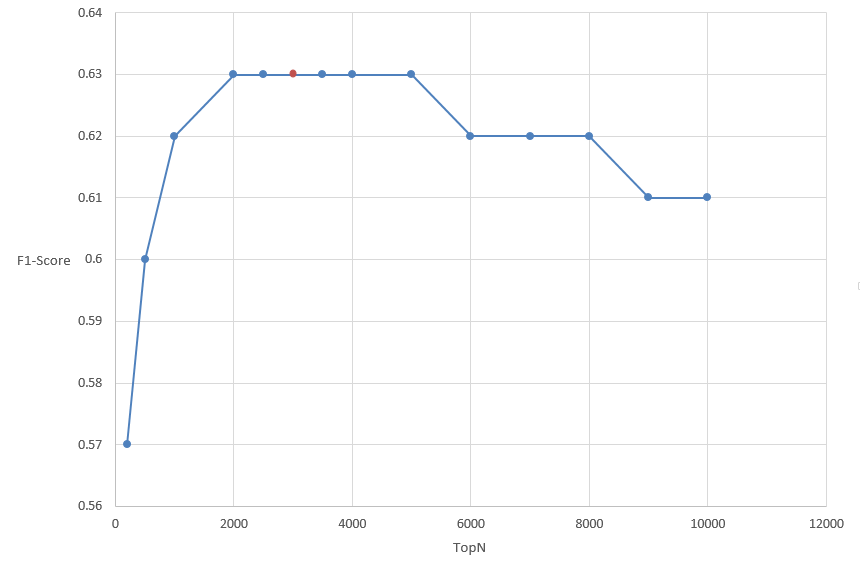
\includegraphics[scale=0.5]{figures/NB.png}}
\caption{Result of Statistic-based Naive Bayes}
\label{fig:basic_NB}
\end{figure}

As we can see in Figure \ref{fig:basic_NB}, this method achieves the best performance when the threshold is set as 2500. At this point, we get a F1-score of 0.63 with a precision score of 0.63 and a recall score of 0.63.

In this method, we also consider the influence of stop words by ignoring the top N words having higher frequences. However, it doesn't make sense. As showed in Figure \ref{fig:start_NB}, although we achieve the best performance when we ignore the top 20 words, the F1-score only improve 1 percentage. When we set the parameter N a little value, such as 50, it even performs worse. That is to say, in our experimental dataset, the most common words are meaningful to the category result.

\begin{figure}[!htb] \centering{
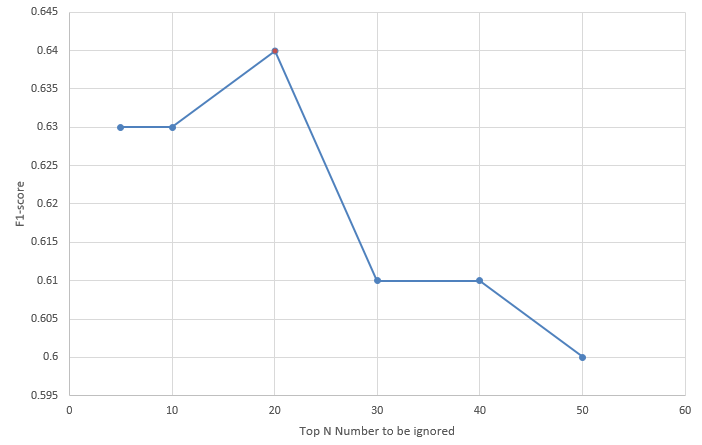
\includegraphics[scale=0.5]{figures/NBStart.png}}
\caption{Result of Statistic-based Naive Bayes Ignoring top N Words}
\label{fig:start_NB}
\end{figure}

\subsection{Mutual Information}
\label{section:MI}
In this method, we use all words' mutual information in a document as the criteria. We formulate it using the Equation \ref{equ:5}.

\begin{equation}
\label{equ:5}
  MI_{avg}(c)=P(c)\sum_{i=1}^n{MI(t_i,c)}
\end{equation}

As the same situation in the method of statistic-based Naive Bayes, the size of document corpus is too big. It has a lot of noises. So we need to pick up the most meaningful ones. In our work, we use the strategy expressed in Equation \ref{equ:4}. We calculate the performance with a different parameter N indicating the number of features, and the result is showed in Figure \ref{fig:MI}.

\begin{figure}[!htb] \centering{
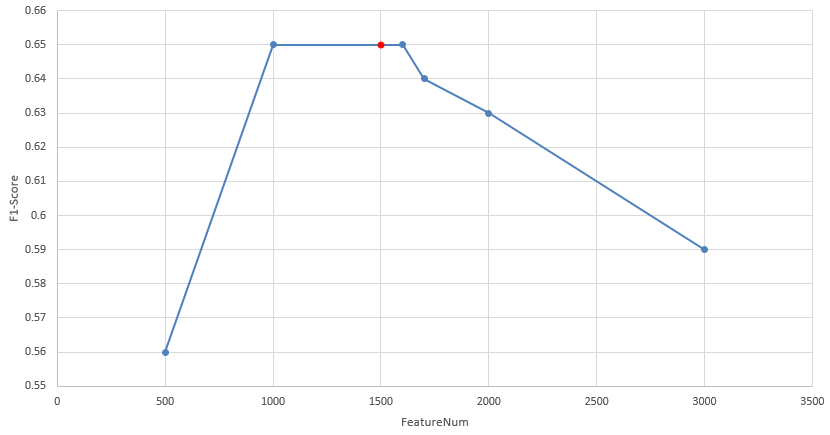
\includegraphics[scale=0.5]{figures/MI.png}}
\caption{Result of Mutual Information}
\label{fig:MI}
\end{figure}

As shown in Figure \ref{fig:MI}, this method achieves the best performance when the number of features is around 1500. And at this point, we get a F1-score of 0.65 with a precision score of 0.55 and a recall score of 0.81.

\subsection{SVM using Mutual Information}
In this method, we use the mutual information as features and try to use SVM to make the classification. Just using the same strategy as Section \ref{section:MI}, we get the selected keywords. However, the mutual information value of each word is calculated in a different way since it needs to include all relatedness with different target categories. Here we use the method defined in Equation \ref{equ:3}.

Firstly we try different parameters which indicates the top number of keywords we used and the result is showed in Figure \ref{fig:SVMMI}. The kernel function we used in Figure \ref{fig:SVMMI} is the linear one, and we can see that it achieves the best performance when the parameter is set as 2000. At this point, it achieves a F1-score of 0.64 with a precision score of 0.76 and a recall score of 0.55.

\begin{figure}[!htb] \centering{
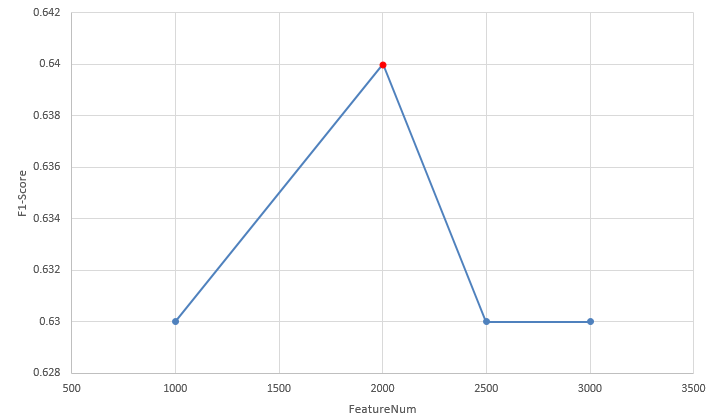
\includegraphics[scale=0.5]{figures/SVMMI.png}}
\caption{Result of SVM Using Mutual Information}
\label{fig:SVMMI}
\end{figure}

At the same time, we adapt several kernel functions to test the performance with the number of keywords set as 2000. As showed in Figure \ref{fig:Kernel}, we try three types of kernel functions. Namely, a sigmoid kernel function, a radial basis function and a linear one. It shows that we get the best performance with the linear one. At the same time, the linear kernel has the best performance on speed.

\begin{figure}[!htb] \centering{
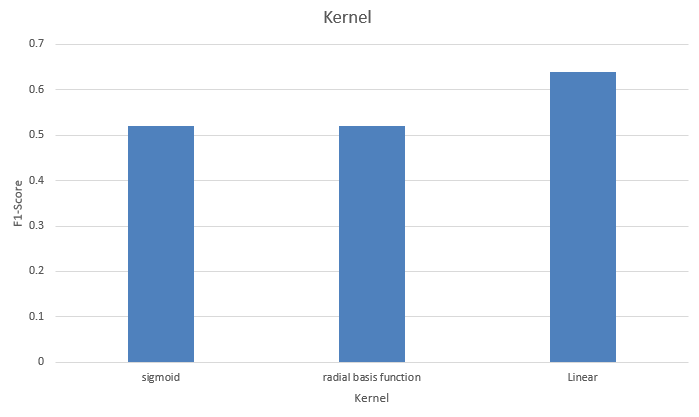
\includegraphics[scale=0.5]{figures/Kernel.png}}
\caption{Result of SVM Using Mutual Information with different Kernel Functions}
\label{fig:Kernel}
\end{figure}

Since we have other information in our data set, such as the like number, the comment number, the retweet number. We make a comparison experiment using these information. Since these features are represented by Integer, we try two methods to represent them. The first one is using a binary value to indicate whether the corresponding number is zero or not, the second one is to normalize them as a percentage. The result is showed in Figure \ref{fig:Information}. We can see that they have little difference. That is to say, compared with the content information of the microblog text, the other information in the data set doesn't make sense.

\begin{figure}[!htb] \centering{
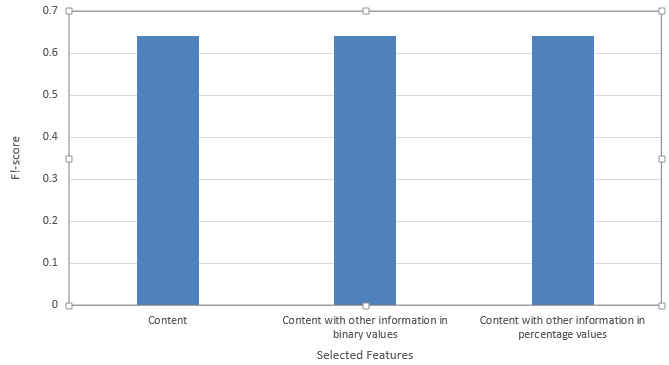
\includegraphics[scale=0.5]{figures/Features.png}}
\caption{Result of SVM Using different features}
\label{fig:Information}
\end{figure}

\subsection{Topic Modeling with SVM}
In the training phase, we get the training data set which contains microblogs and corresponding labels.

Firstly we train a topic model using LDA method, then we get $K$ topics and corresponding topic distributions with regard to microblogs.
For each microblog, we generate a $K$-dimensional vector from the topic distribution.
The value of each element in the vector is $P(t_k|m_i)$ which means the probability of the $i$th microblog belonging to the $k$th topic.

After topic modeling, we use a classifier to train a model with the $K$-dimensional topic feature vector.
In our settings, SVM classifier is used and we choose the linear kernel.

\begin{figure}
\centering
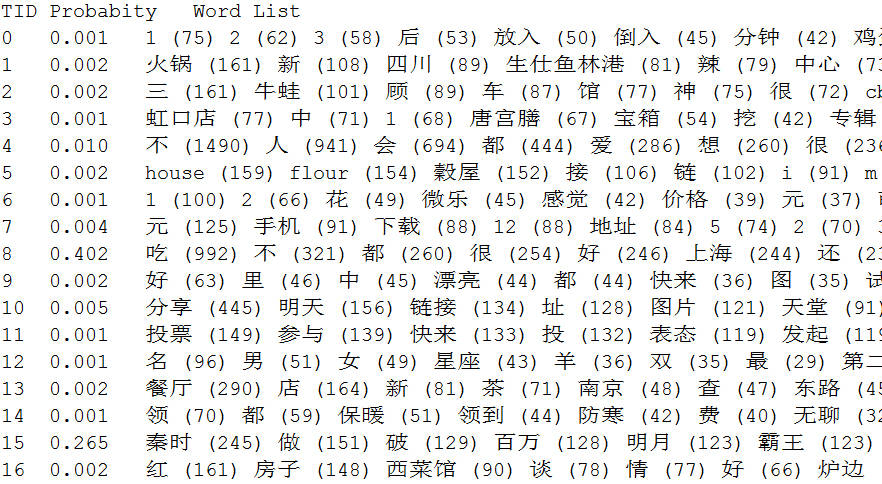
\includegraphics[scale=0.5]{figures/topic.png}
\caption{Topic with High Probability Words}
\label{fig:topics}
\end{figure}

The abstract topics generated by topic modeling is shown in Figure \ref{fig:topics}.
Each topic is followed by a list of top 10 words with regard to $P(t_k|w_n)$.
The first column is the topic ID. And the second column is the distribution probability for the given topic against this microblog.

\begin{figure}
\centering
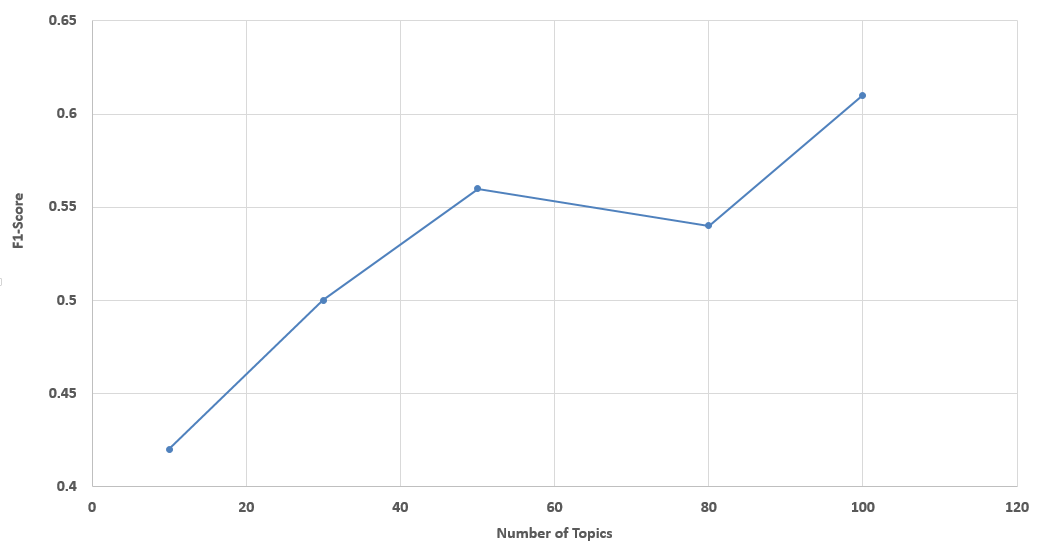
\includegraphics[scale=0.4]{figures/topic-num.png}
\caption{Performance with Topic Number}
\label{fig:topic-num}
\end{figure}

\begin{figure}
\centering
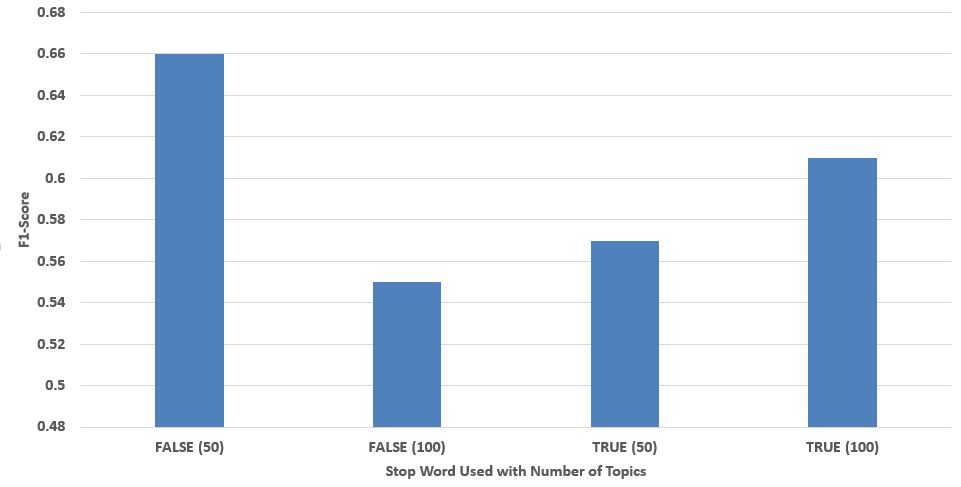
\includegraphics[scale=0.4]{figures/stopword.png}
\caption{Performance with Topic Number}
\label{fig:stopword}
\end{figure}

In Figure \ref{fig:topic-num}, the result shows the diversification of accuracy with regard to different topic numbers.
Here we may find that the topic number has great influence on classification performance.
10 topics is not sufficient. So we set the topic number as 100 in the final test.

At first, we use stop word list to filter out those words which appears very frequently.
Figure \ref{fig:stopword} shows the performance with and without stop word removal operation.
However we may find that the performance without stop word removal is better than removing stop words with topic number set to 50.
When topic number is set to 100, the performance shows that stop words play some important role in training.

\begin{figure}
\centering
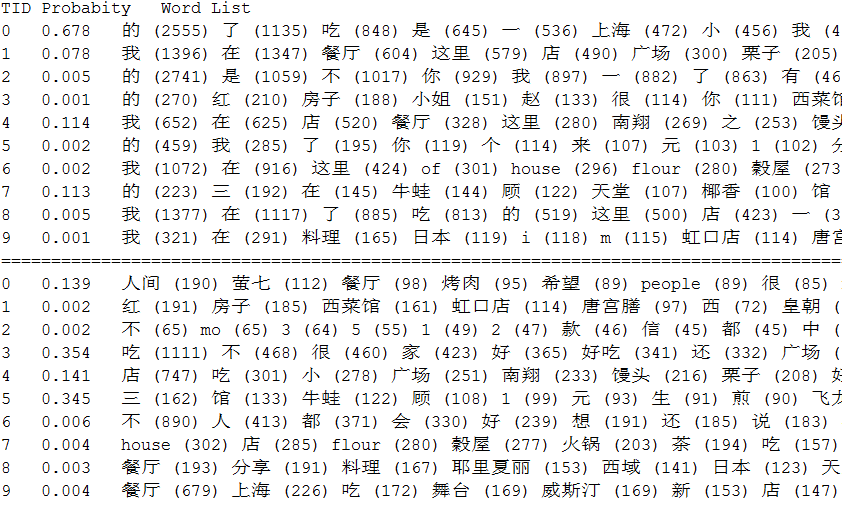
\includegraphics[scale=0.45]{figures/topics-stopword.png}
\caption{Performance with Topic Number}
\label{fig:topics-stopword}
\end{figure}

Figure \ref{fig:topics-stopword} shows different word list of topics, with regard to stop words removal or not.
The upper part of the word list is learned without stop word removal and the bottom part is learned with stop word removal.

\begin{figure}
\centering
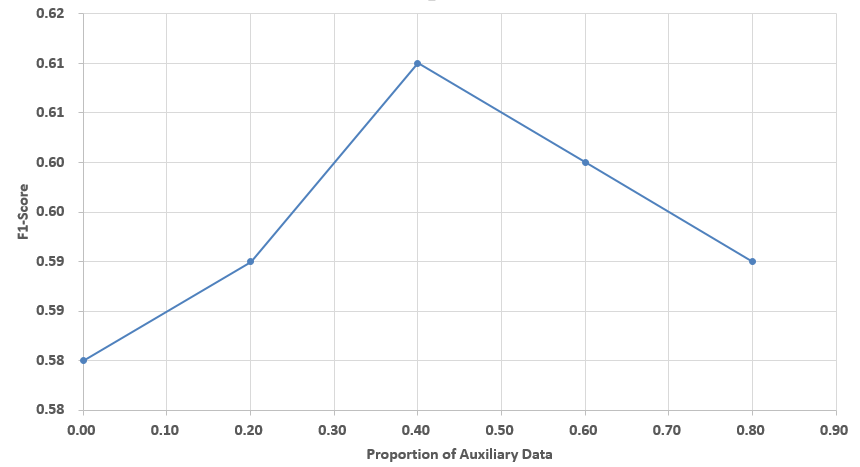
\includegraphics[scale=0.45]{figures/auxiliary.png}
\caption{Performance with Auxiliary Data Proportion}
\label{fig:auxiliary}
\end{figure}

Moreover, we find that all the training data set is about restaurants.
Intuitively, we want to model different abstract topics over more general microblogs.
So that we add some general microblog data along the timeline.
The size of the auxiliary data is proportional to the training data set.
And the proportional ratio is set as a parameter $r,~0\leq r \leq 1$.
Figure \ref{fig:auxiliary} shows the performance of different size of auxiliary data set.
We may find that more auxiliary data (until 0.4 with regard to training data set) makes better performance, though the improvement is not large.
And adding more auxiliary data (more than 0.4) has reverse influence.

\begin{figure}[!htb]
\centering
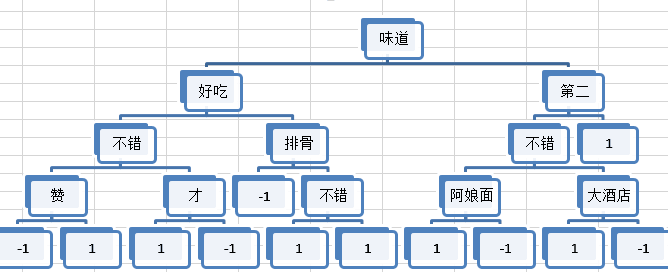
\includegraphics[scale=0.45]{figures/tree.png}
\caption{Decision Tree}
\label{fig:tree}
\end{figure}

\subsection{Decision Tree}
Figure \ref{fig:tree} shows the decision tree we obtained.
The left side direction of each decision is negative, otherwise on the right side.
Label ``-1'' means the model classify the  data as non a review while ``1'' as true review.

\subsection{Overall}

Overall, all the performance of our models are listed in Table \ref{tab:performance}.
Here we can see that all of our methods preform better compared with the baseline. And also, different methods achieve similar performance considering the F1-score. Naive Bayes achieves balance performance between the precision score and the recall score, Mutual Information and Topic Model with SVM achieve higher recall scores, while SVM using Mutual Information and Decision Tree achieve higher precision scores.

\begin{table}[!hbp]
\caption{Overall Performance}
\label{tab:performance}
  \setlength{\tabcolsep}{12pt}
  \begin{tabular}{|c|c|c|c|}
  \hline
  Method&Precision&Recall&F1-Score\\
  \hline
  Baseline&0.30&1.0&0.46\\
  \hline
  Naive Bayes & 0.63 & 0.63 & 0.63\\
  \hline
  Mutual Information & 0.55 & 0.81 & 0.65\\
  \hline
  SVM using Mutual Information & 0.76 & 0.55 & 0.64\\
  \hline
  Decision Tree & 0.83 & 0.41 &0.55 \\
  \hline
  Topic Model with SVM & 0.59& 0.73& 0.66\\
  \hline

  \end{tabular}
\end{table}


\section{Discussion}
In our work, we design several methods to extract features from the natural language text. And meanwhile, we try different models combined with our selected features to evaluate our methods. The final results show that all of the methods make sense. That is to say, the feature selection method works well. 

Our method achieves a F1-score of 0.65. One of the reasons may be that the training data set is not enough, we have less than ten thousand texts in total. We need to adapt the training data to calculate the word frequences and document frequences, which depends closely on the training document corpus. So when the data is bigger, our methods may work better. In the other hand, Since all of the different models we use achieve similar performance, the work we need to do in the future should also focus on the work of feature selection. We will try more feature selection methods about text classification in the future. 

\bibliographystyle{llncs2e/splncs03}
\bibliography{paper}
\clearpage

\end{document}
